\documentclass{elsarticle}

\usepackage[utf8]{inputenc}

\title{A Refined Wave Resource Assessment Methodology: Application to U.S. Waters}
\author{Levi Kilcher, Gabriel-Garcia Medina, Zhaoqing Yang, Aidan Bharath}
\date{October 2019}

\showboxdepth=5
\showboxbreadth=5

\begin{document}
\maketitle


\begin{abstract}
Test this
\end{abstract}

\section{Introduction}

Over the last decade global interest in wave energy has grown considerably, with the Ocean Energy Systems executive committee setting a goal of 300GW of installed ocean energy capacity by 2050 (International Energy Agency 2017). This has been driven by concerns about greenhouse-gas driven climate change, carbon-based energy price volatility, and a growing understanding of the value of diversifying energy sources. Wave energy technology is still at an early-stage of technology development, with a wide-range of device archetypes under active development (Babarit 2017).
During these early years of wave energy research and development, it has been important to quantify the wave energy resource so that decision makers can understand the market opportunity of this new technology. Wave energy resource assessments can be divided into two types:
Global, regional, and national assessments (hereafter, collectively ‘regional’ assessments) that quantify the total theoretical resource for a relatively long section of coastline (i.e., $>$O(100 km)). Most importantly, regional assessments provide an estimate of the total power available in the wave field for the region of interest.
Site resource assessments provide a collection of resource details that are useful for estimating the site’s power production potential and for project design. Most importantly, site assessments provide a joint probability distribution of wave energy period and wave height that can be used with a device ‘power matrix’ to calculate the project’s annual energy production.
These assessments are valuable for different purposes. Regional assessments are the foundation of more detailed market research (such as site assessments), they motivate regional planning, and provide justification for government investment \citep[e.g., ][]{EPRIwaveresource2011,gunnQuantifyingGlobalWave2012}
(Jacobson et al. 2011; Gunn and Stock-Williams 2012; Reguero et al. 2015; Mota and Pinto 2014). Site assessments provide data needed for feasibility and design studies that are critical to obtaining project financing and investment (Robertson, Hiles, and Buckham 2014; Iglesias and Carballo 2009). 

The methodologies of these assessment types are currently distinct because the marine energy community has not yet developed a unified assessment method that provides the data for both (large-scale total energy-flux and also the power matrix at a site). 
A detail that confounds unifying these two approaches is the fact that wave energy flux is a directional quantity. This means that - in order to avoid double counting - regional totals must account for the directionality by performing a line-integral. On the other hand, for site assessments involving sparsely positioned omni-directional devices (i.e., devices that absorb energy equally in all directions), wave directionality does not have a significant impact on the project’s technical potential. With this understanding and motivated by a desire to address the needs of the industry where it is now (i.e., most projects involve 10 or less devices), the first edition of the International Electrotechnical Commission’s resource assessment technical specification does not explicitly account for directionality or array effects \citep[]{internationalelectrotechnicalcommissionPart101Wave2015}. While the IEC site assessment methodology has these limitations, it has been developed through a consensus process that encourages widespread adoption and consistency. The methodology for regional assessments, on the other hand, has not been developed by consensus, which has led to inconsistent approaches and confusion when comparing results.

We undertake the task of establishing a consistent regional wave resource assessment methodology by first pointing out that the wave resource for a region of water is composed of two parts (Figure 1): 1) the ‘remote resource’, which is the wave energy created by winds outside the region — e.g., by storms in the distant open-ocean — that propagates into the region (Gunn and Stock-Williams 2012; Hemer et al. 2017), and 2) the ‘local resource’, which is the wave energy created by winds within the region itself. The majority of existing wave resource assessments have considered the remote resource only. While neglecting the local resource may be valid in specific scenarios, the fact that it has been ignored (often implicitly) has raised many questions and led to confusion about wave resource assessment methodology. The primary objective of this work is to quantify both the remote and local resource explicitly, and thereby resolve lingering questions regarding the details of regional resource assessment.

\begin{figure}[ht]
  \centering
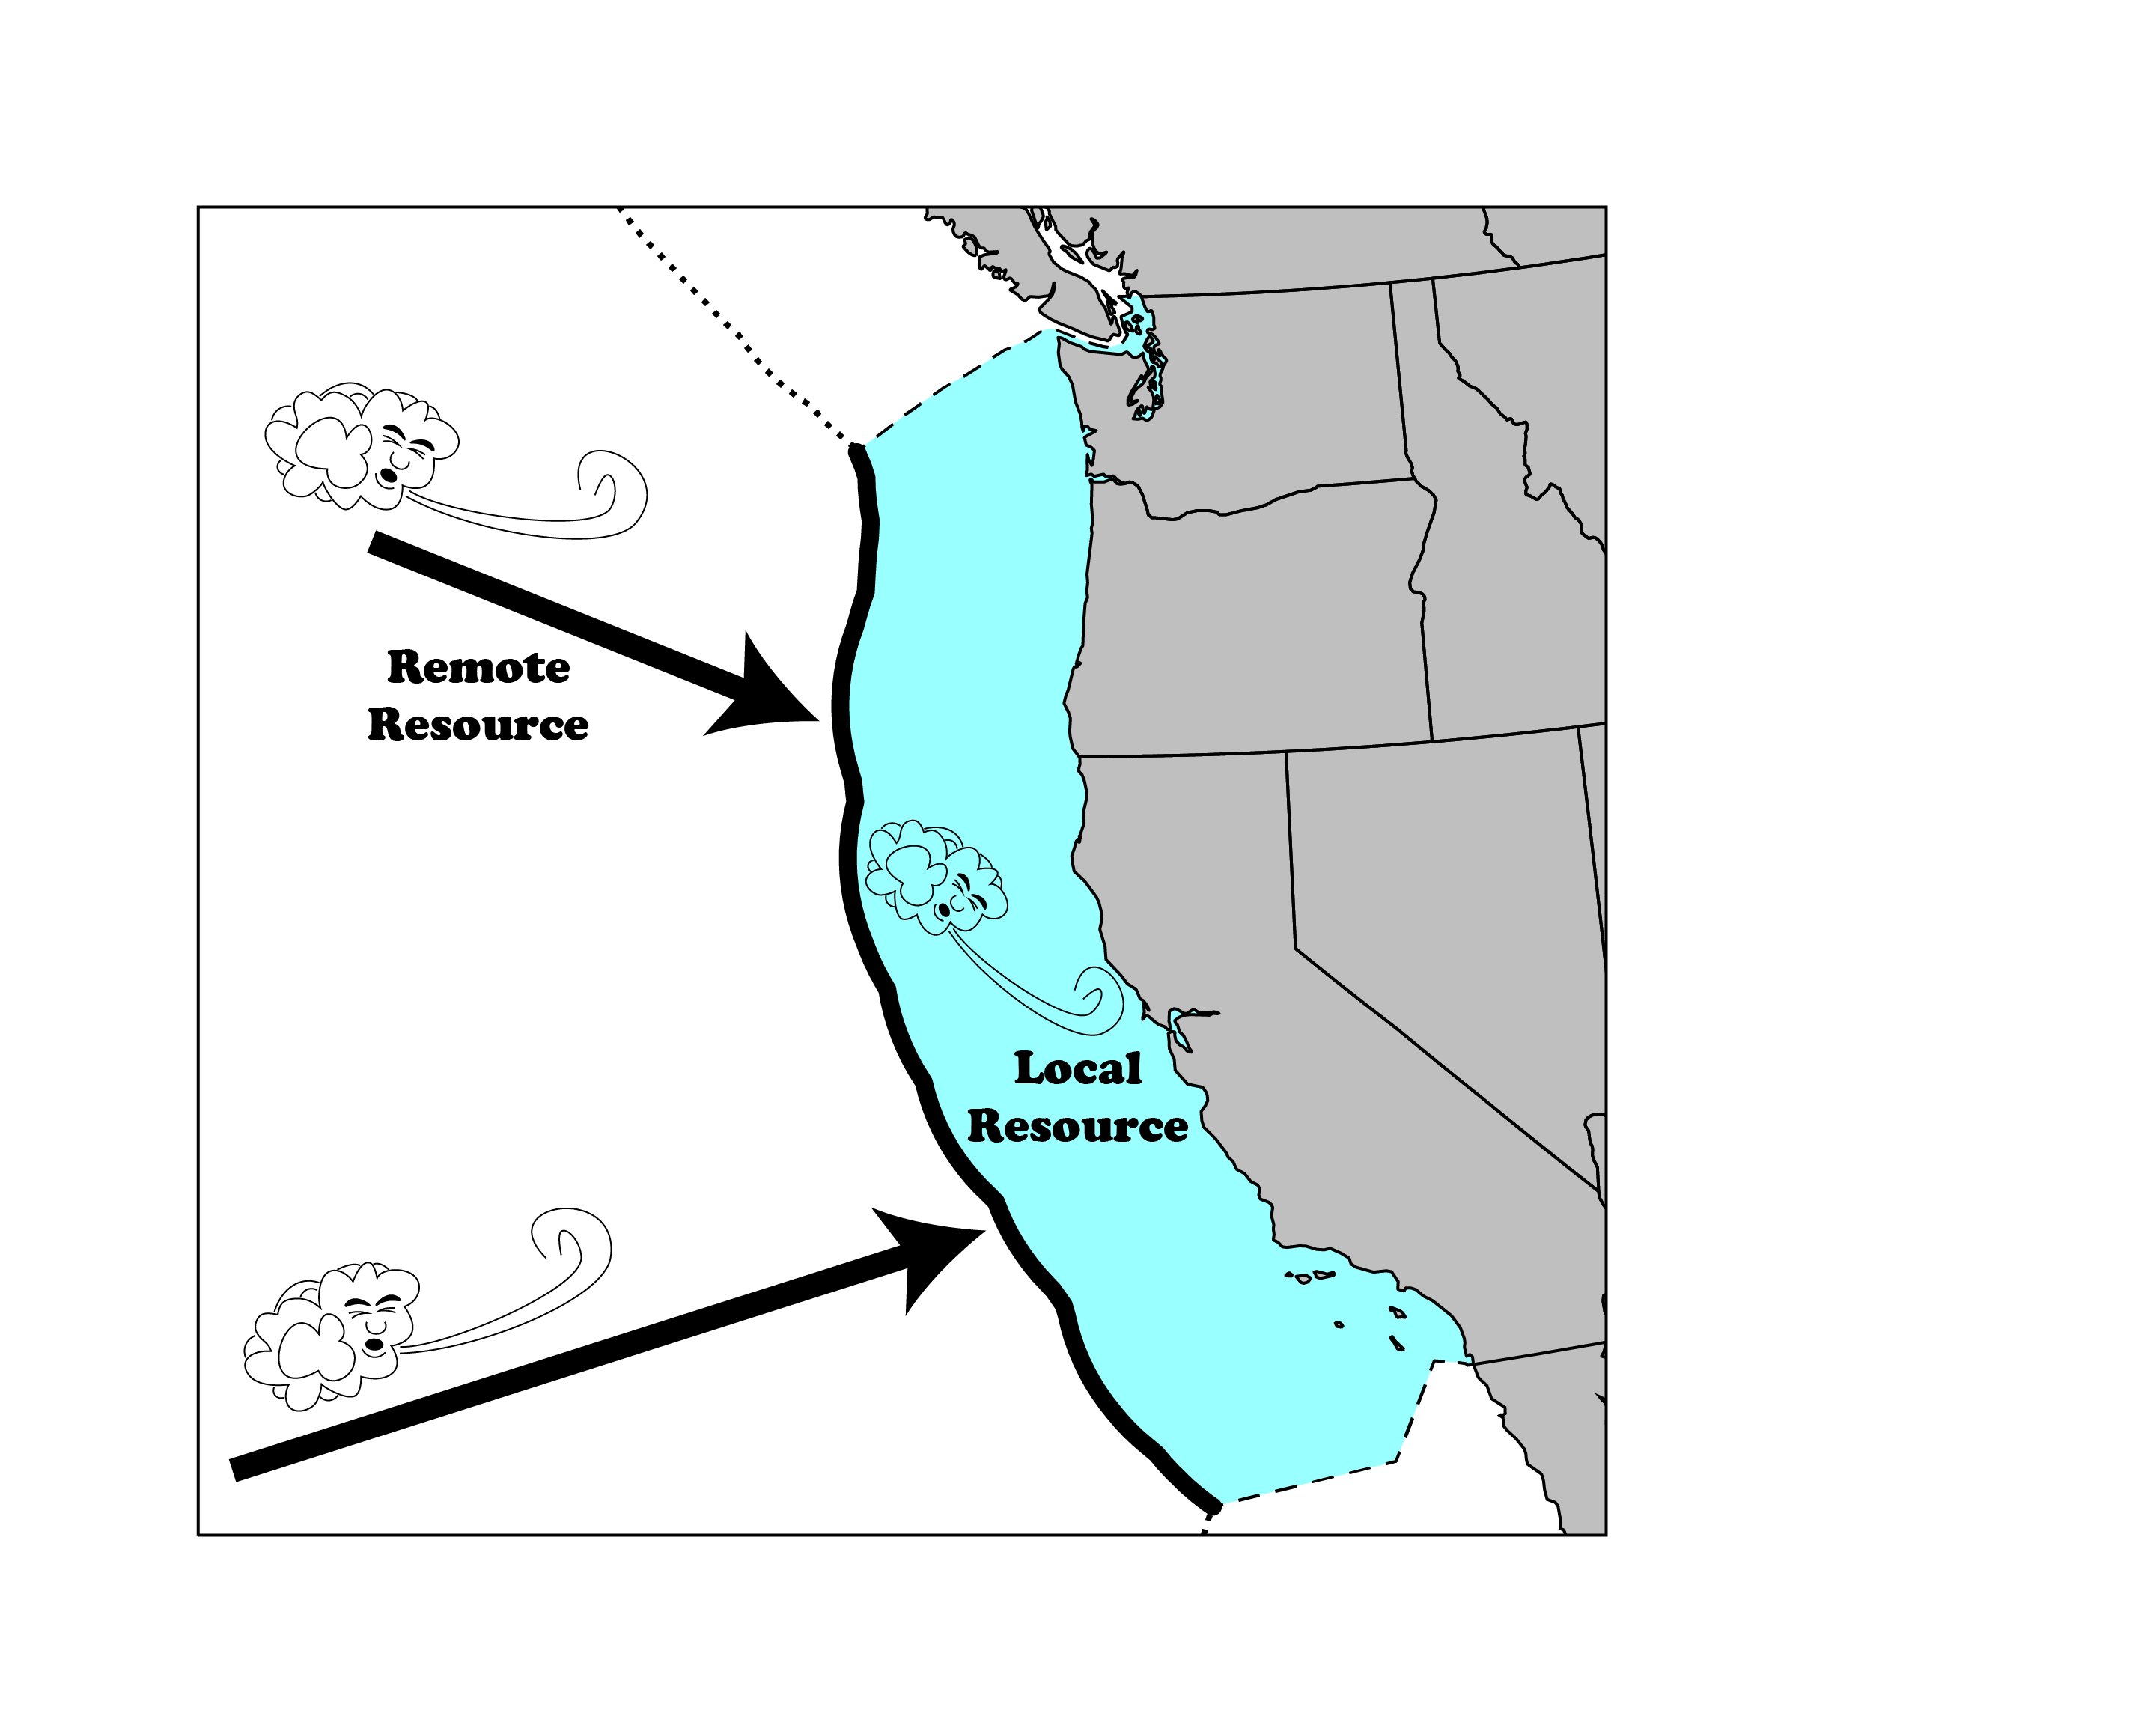
\includegraphics[width=0.9\linewidth]{../diagram/EEZ_contour03_edit01.png}
  \caption{A diagram depicting the U.S. West Coast’s ‘remote’ (arrows) and ‘local’ (cyan) resource.}
  \label{fig:map01}
\end{figure}

A secondary objective of this work is to provide a refined estimate of the U.S. wave resource based on this new method, and new model results. A tertiary objective is to provide guidance that helps address limitations in site assessment, which we hope will eventually lead to a unified methodology for site and regional wave resource assessment.
These objectives are accomplished by first discussing the details of regional assessments (section 2), and then presenting our proposed approach (section 3). In section 4, we present the results of this approach applied to each region of the U.S. coastline in comparison to alternate methods that have been used. Section 5 provides a detailed discussion of the results, including a justification for the proposed approach, and a summary of how the proposed approach can be applied in different scenarios. We conclude with a summary of results, the proposed methodology, and a view toward how to unify wave energy site and resource assessment.

\section{Method}

\clearpage

\bibliographystyle{elsarticle-harv}
\bibliography{Refs}


\end{document}
